\documentclass{article}
\usepackage{graphicx} % Required for inserting images
\usepackage[paperwidth=8.5in, paperheight=11in]{geometry}

\begin{document}
\begin{center}
    
\includegraphics[]{Logo.png} \\
    \Large \textbf{SUPERVISED BY:} \\
     Prof. Nazeef Ul Haq \\
    \textbf{SUBMITTED BY:} \\
    Waleed Ahmed 2022-CS-41 \\
    \textbf{SUBJECT:} \\
    Lab 06 Hometask \\
    \textbf{SECTION:} \\
    A
    \newpage
    In this report, I have displayed how you can create and use stored procedures for an optimized usage in your database: \\
    As you can see, currently there isn't any stored procedure currently present in the stored procedure directory. You can create a stored procedure using \textbf{CREATE storedprocedurename AS SQL Query} \\
    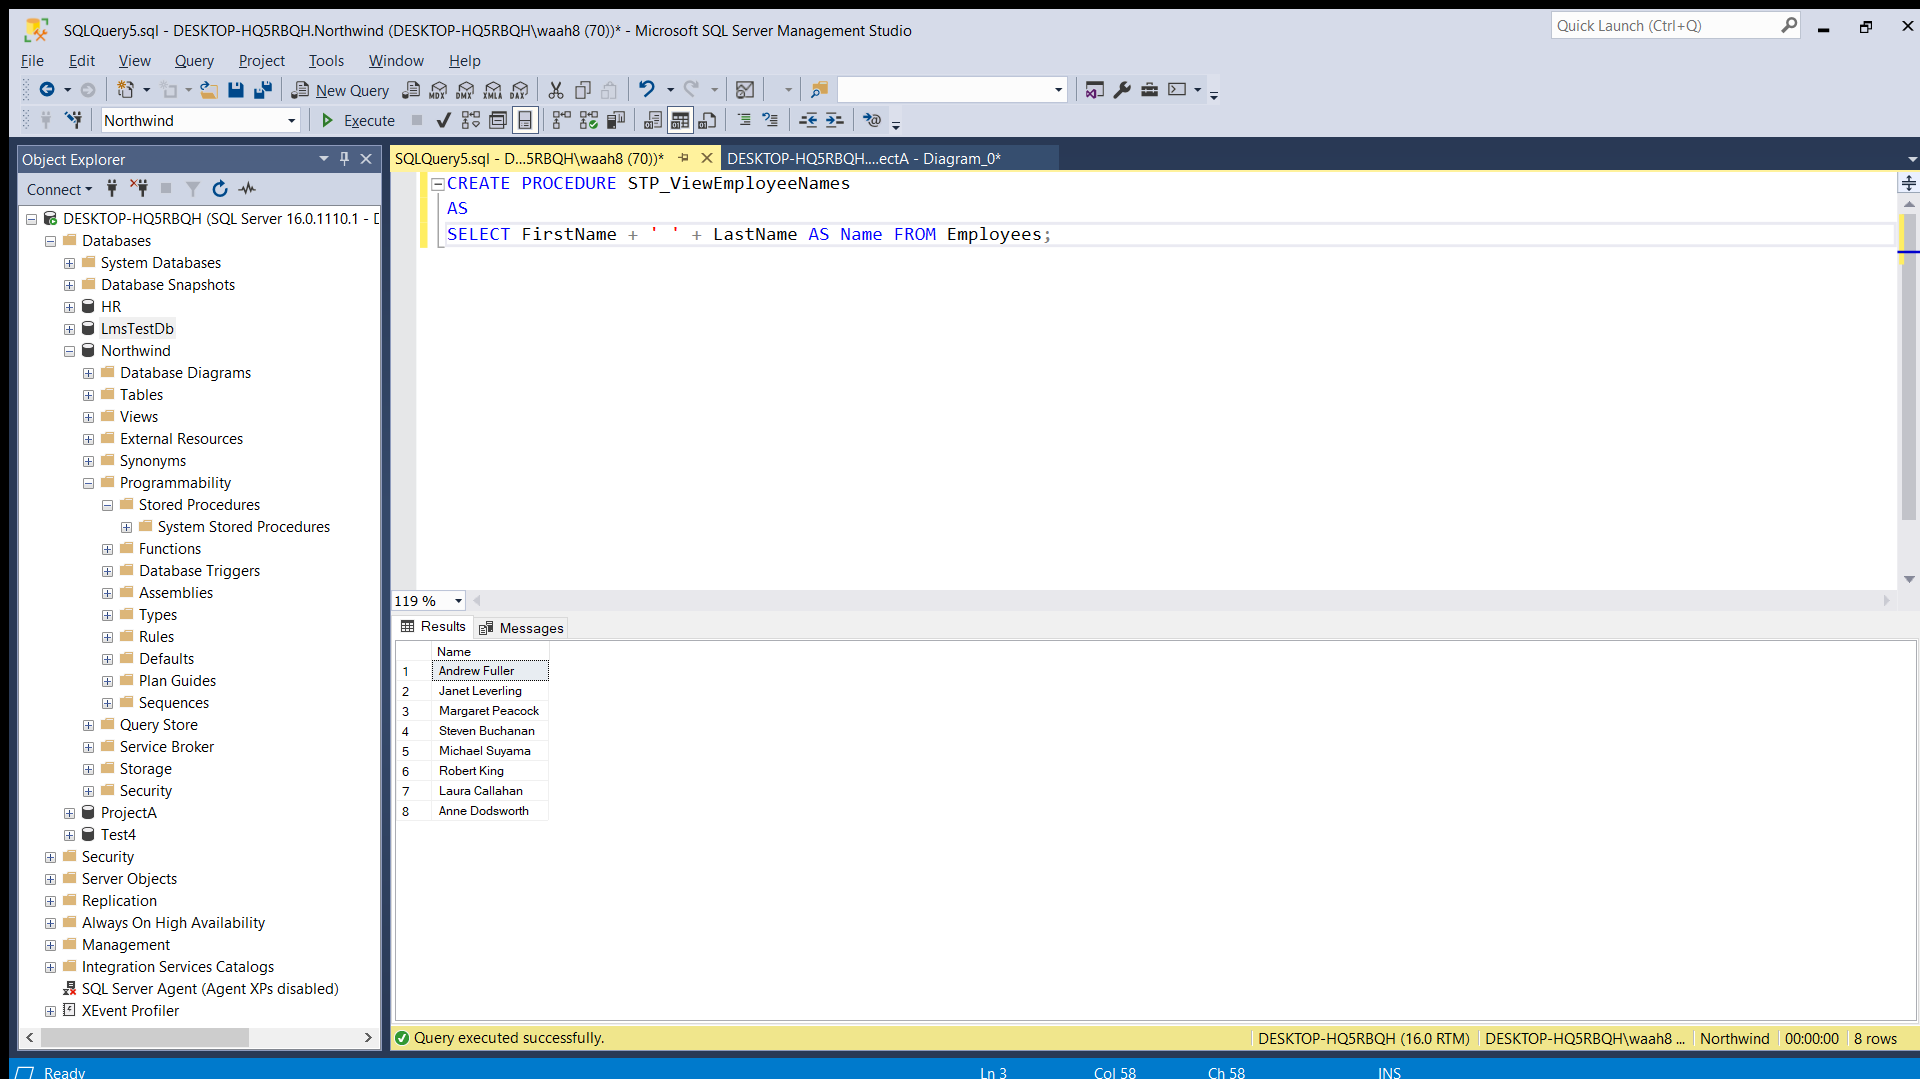
\includegraphics[width=1\textwidth]{1.png} \\
    \newpage
    After I execute the written query you may need to refresh the database directory in order to view the created stored procedure. \\
    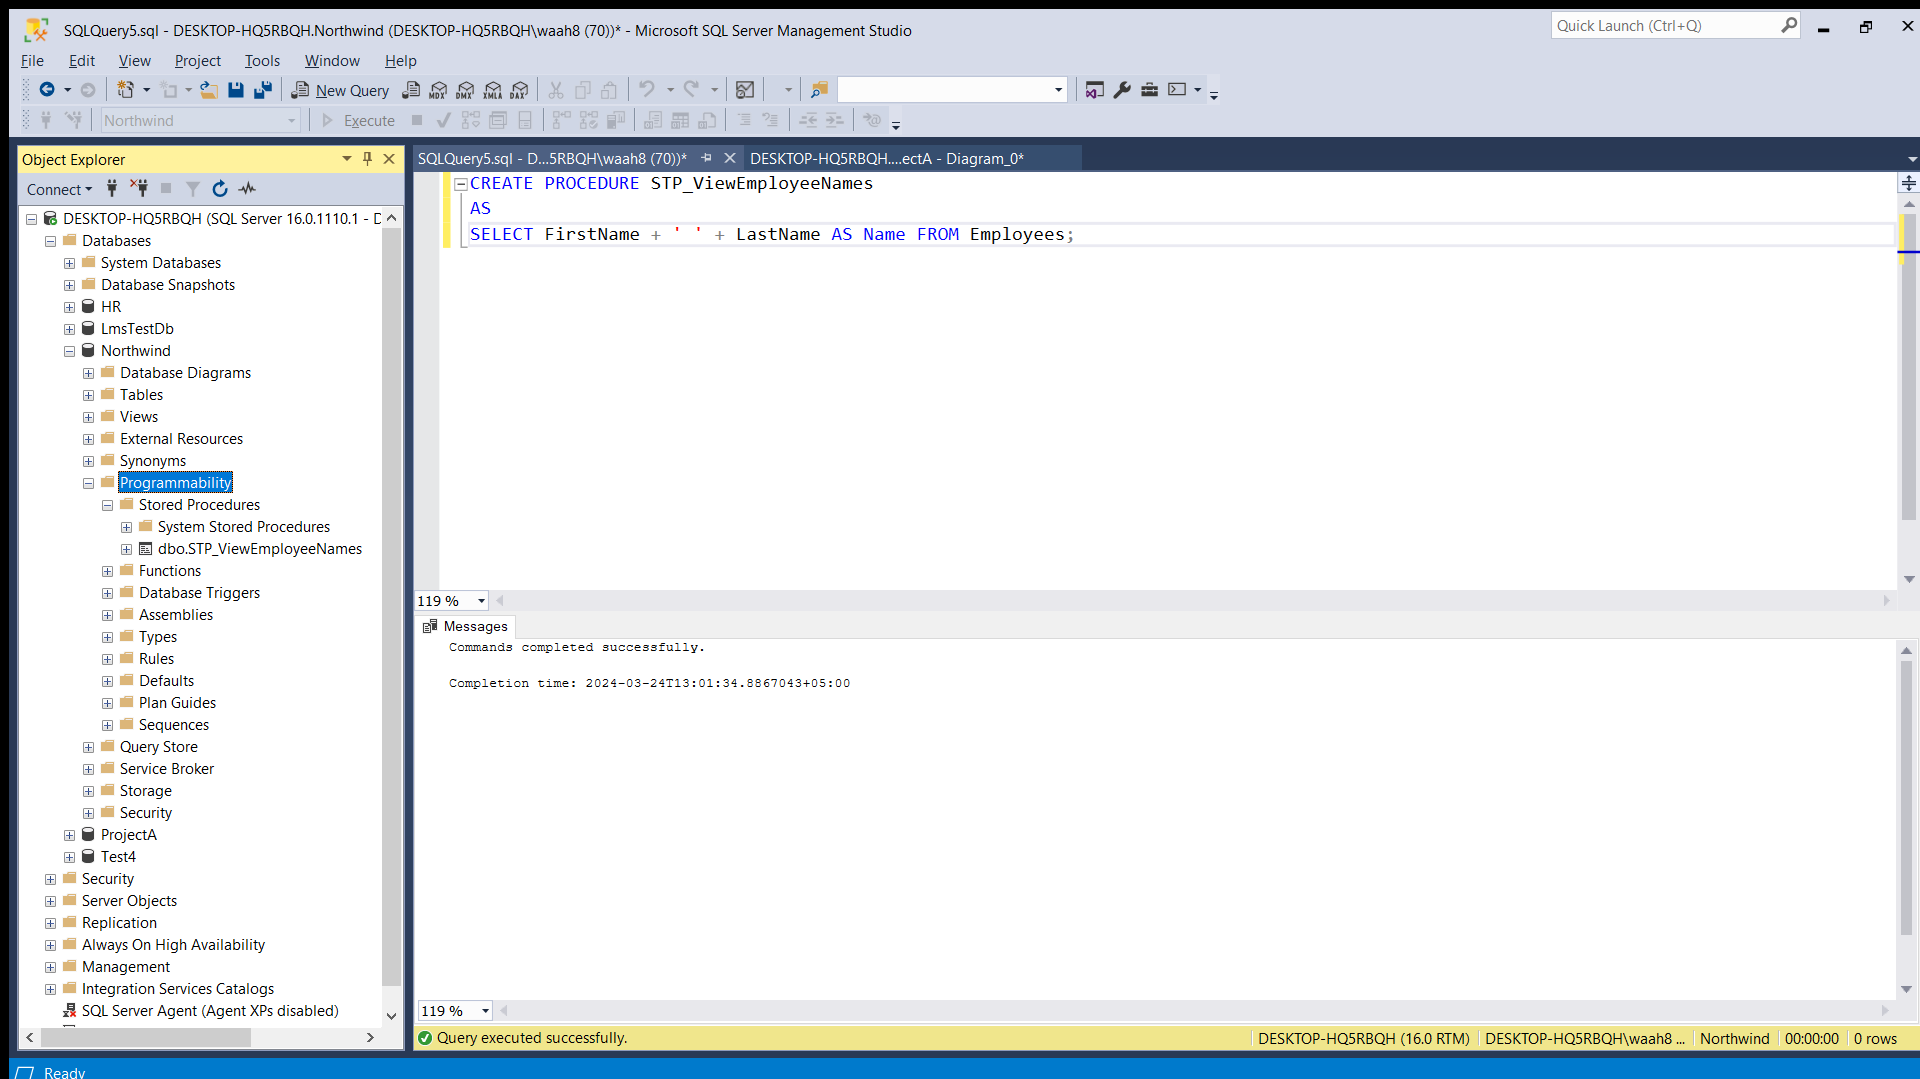
\includegraphics[width=1\textwidth]{2.png} \\
    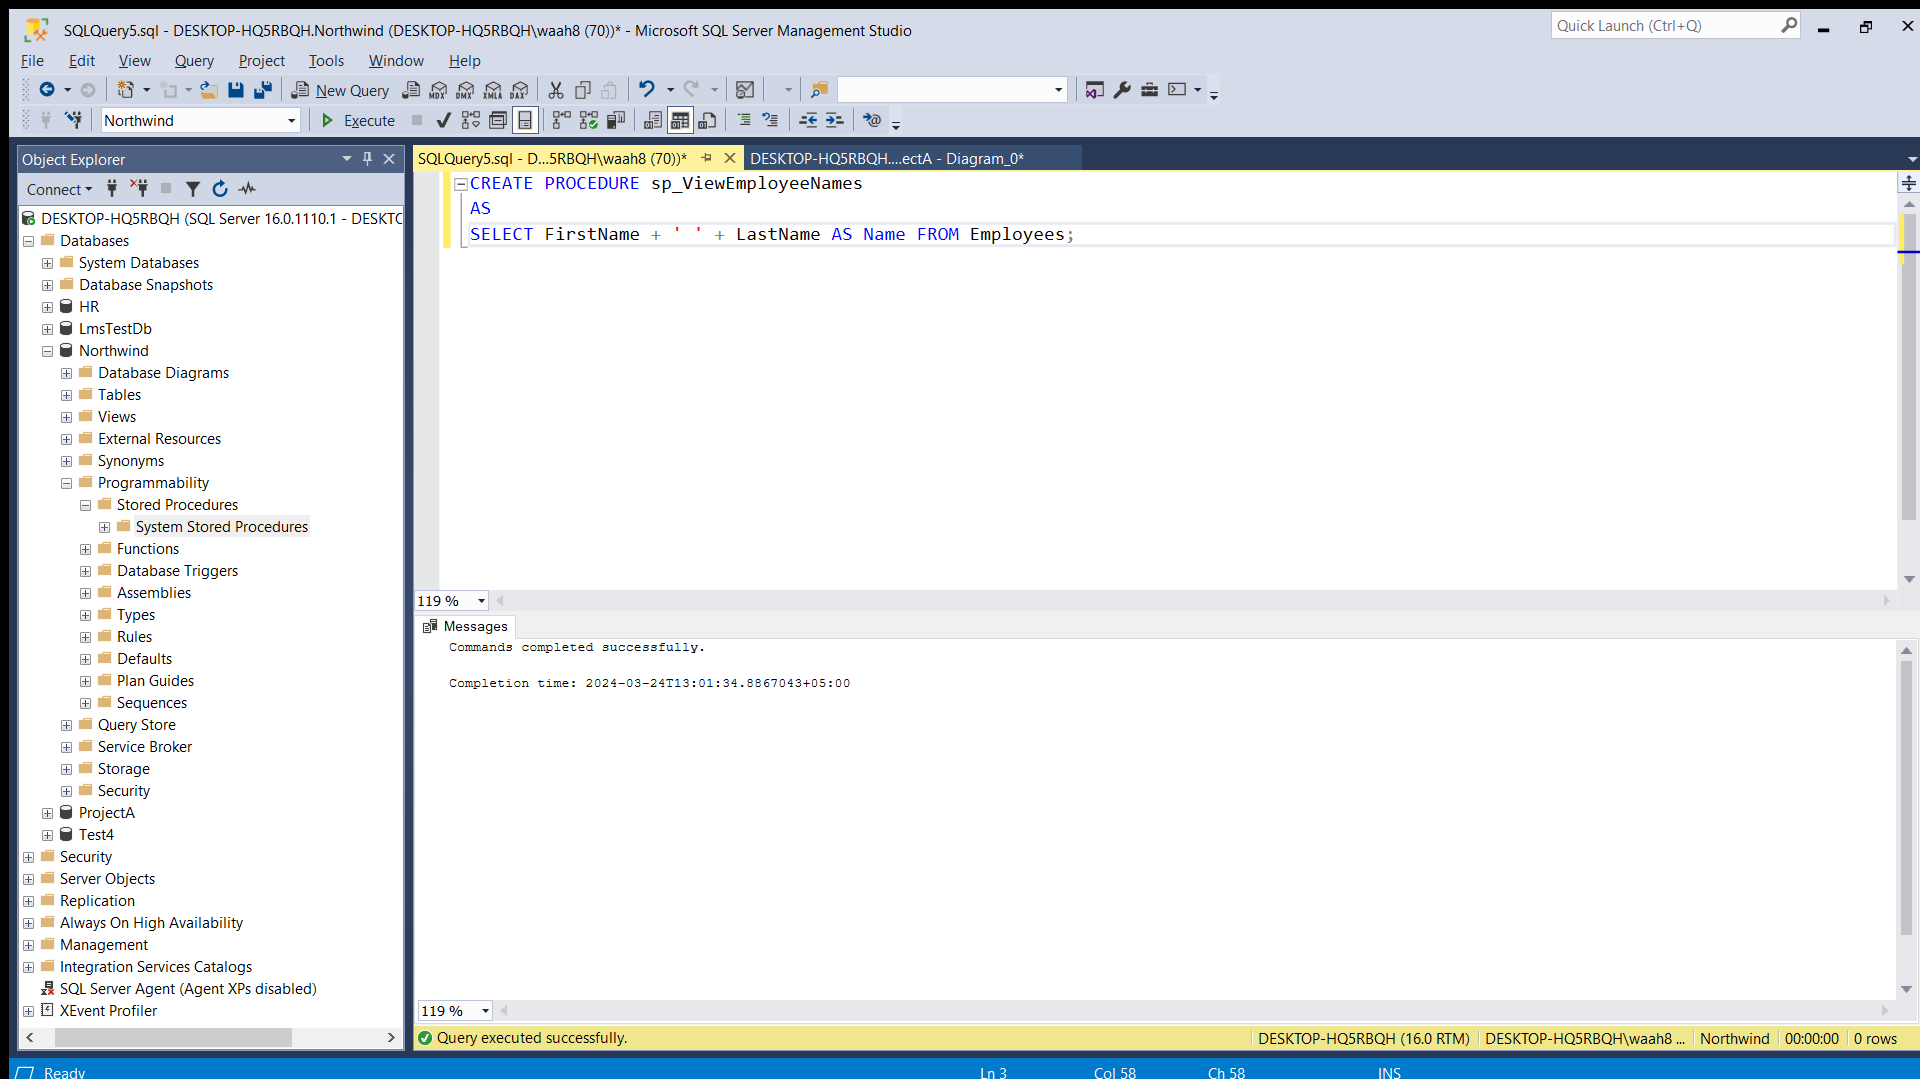
\includegraphics[width=1\textwidth]{3.png} \\
    \newpage 
    Now after successfully creating a stored procedure we can use it by using 
 \textbf{EXEC procedurename} \\
    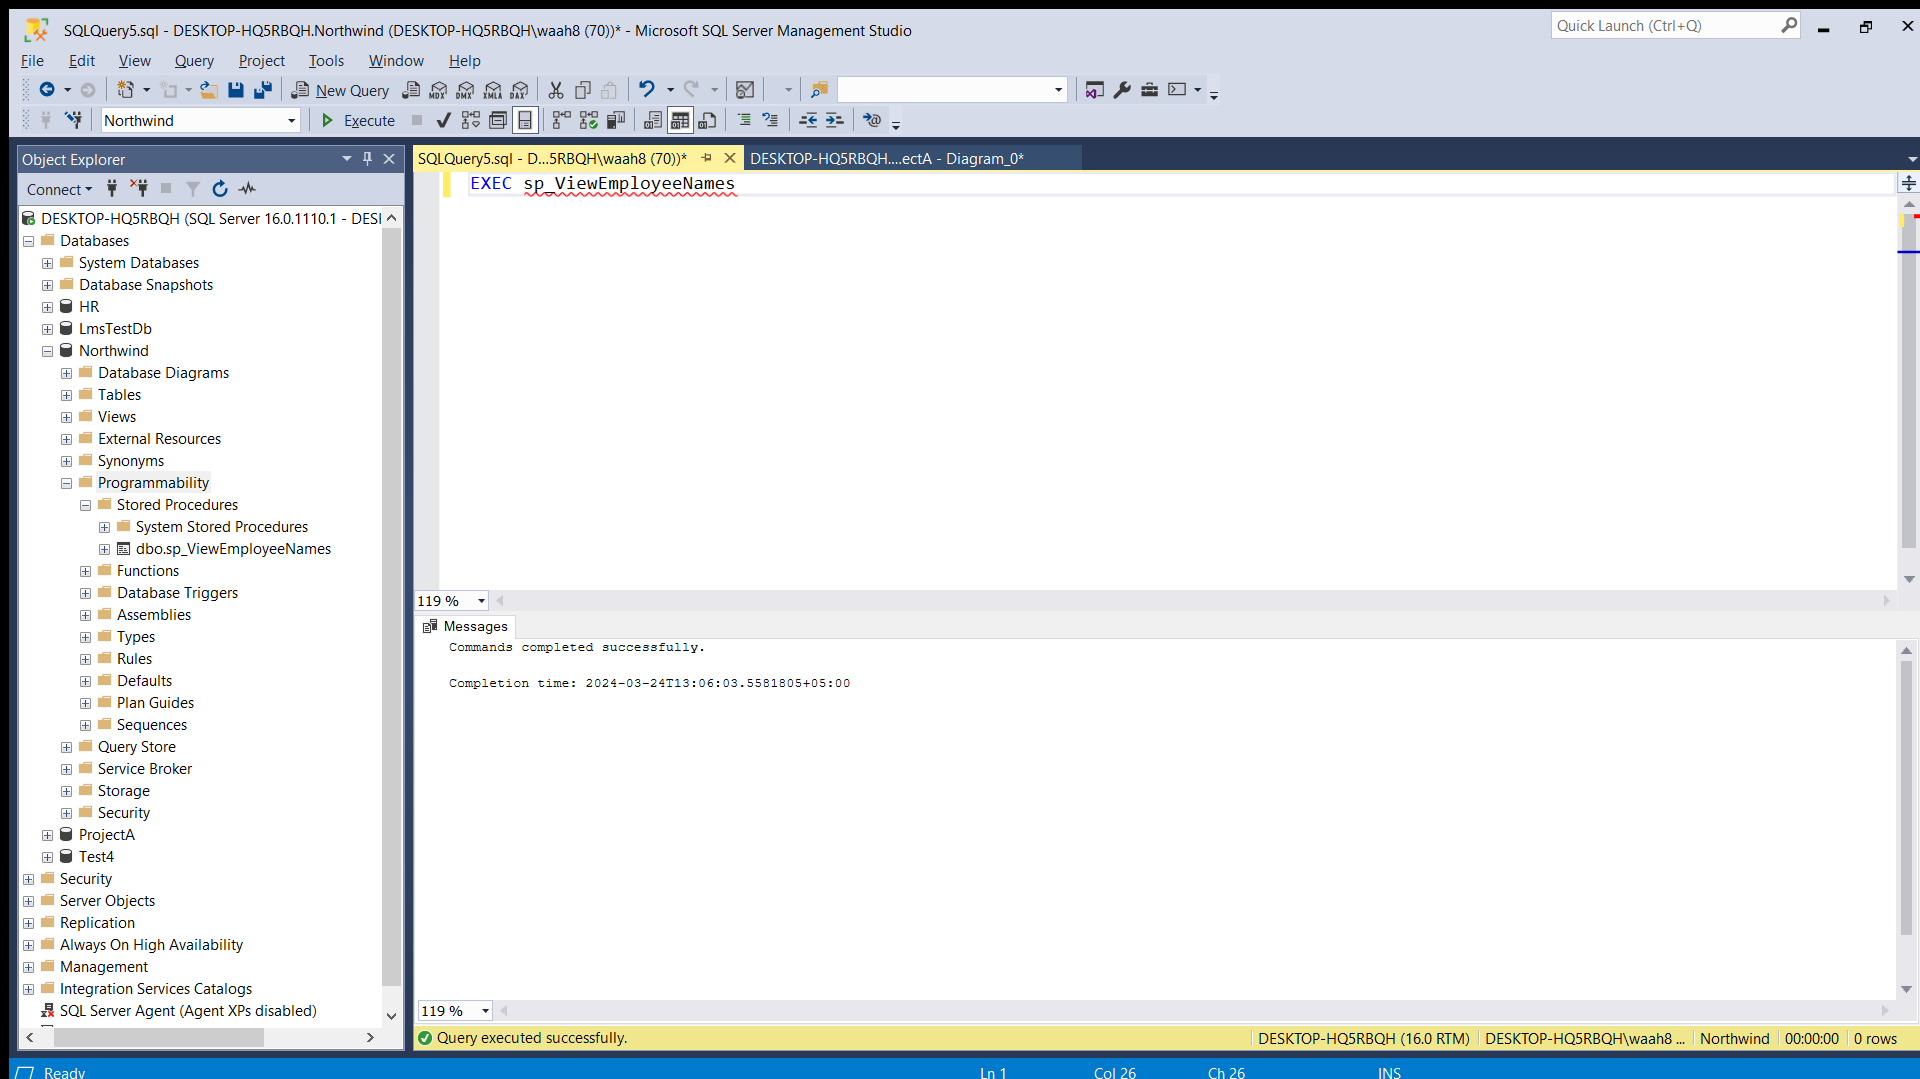
\includegraphics[width=1\textwidth]{4.png} \\
    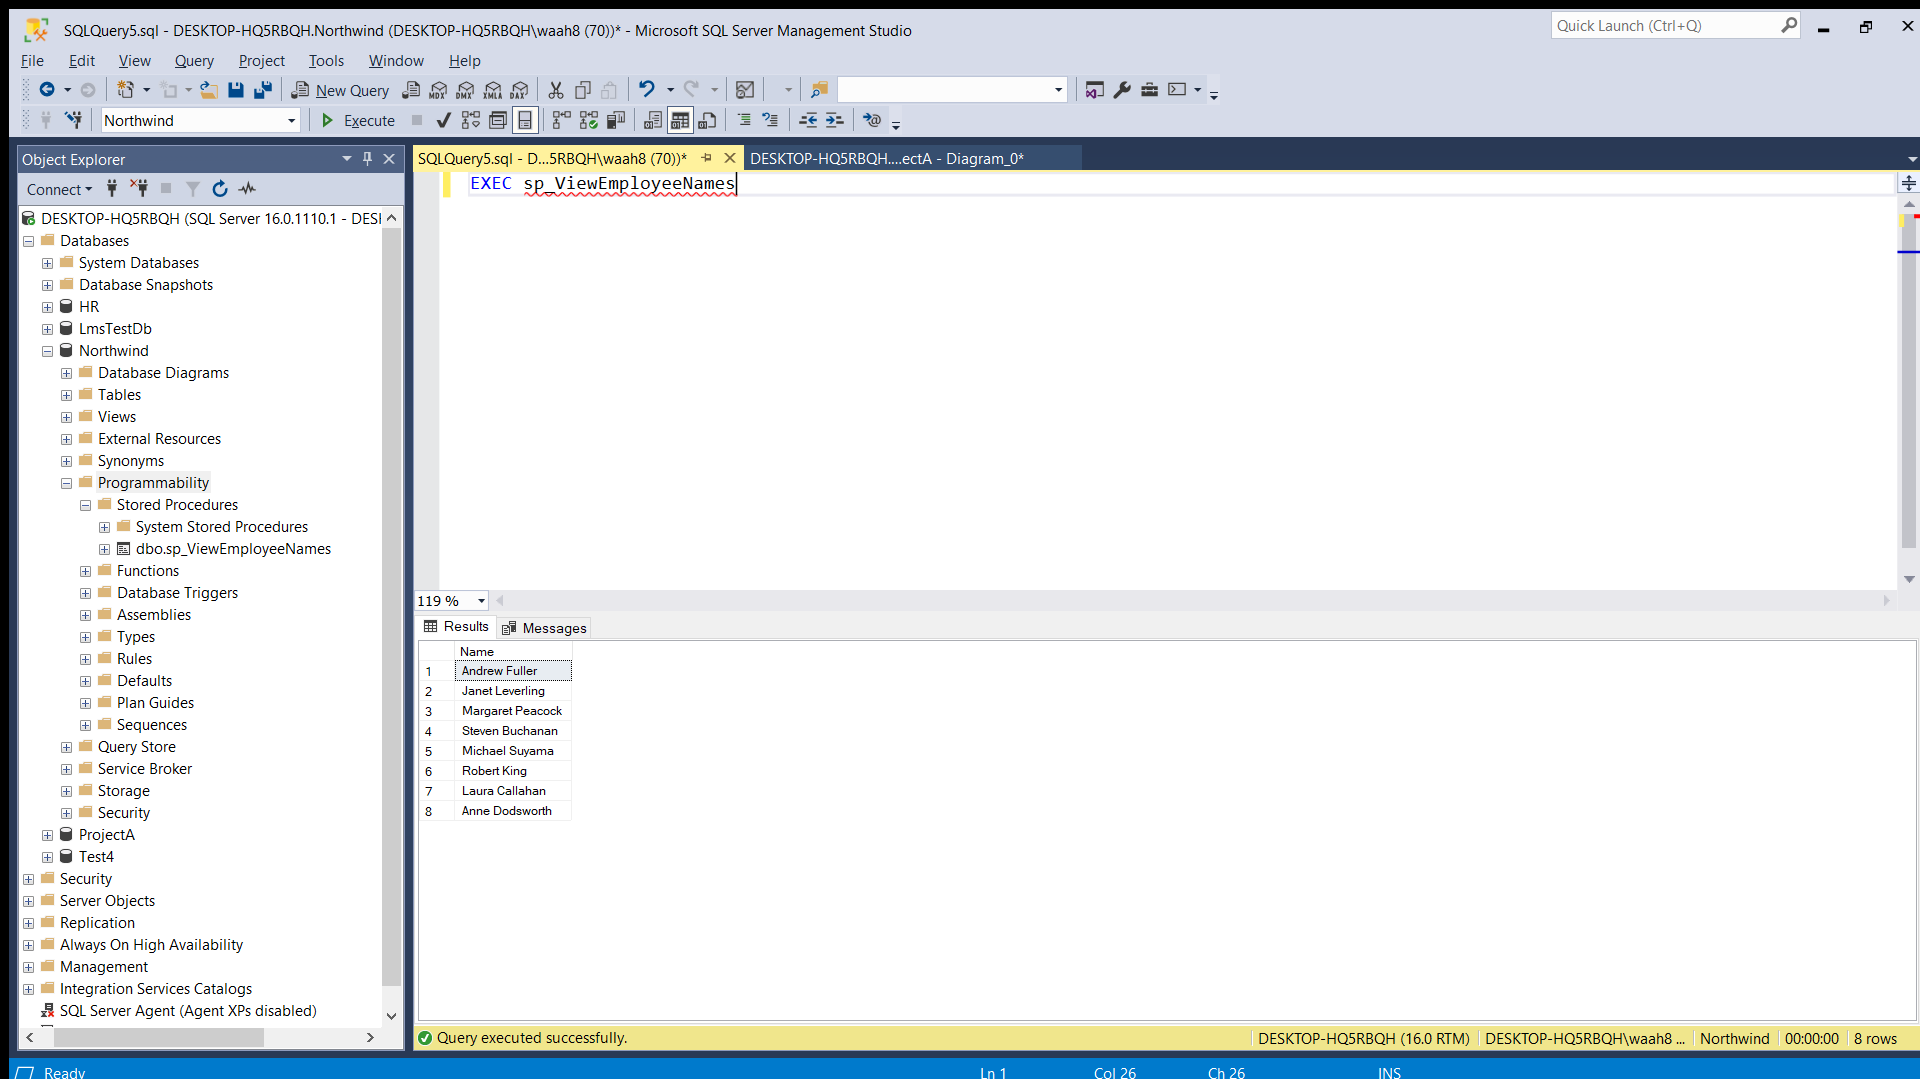
\includegraphics[width=1\textwidth]{5.png} \\
    \newpage
    You can also use stored procedures to create certain table as per desired by the database requirements by using \textbf{CREATE OR INSERT INTO tablename} functions of database.\\
    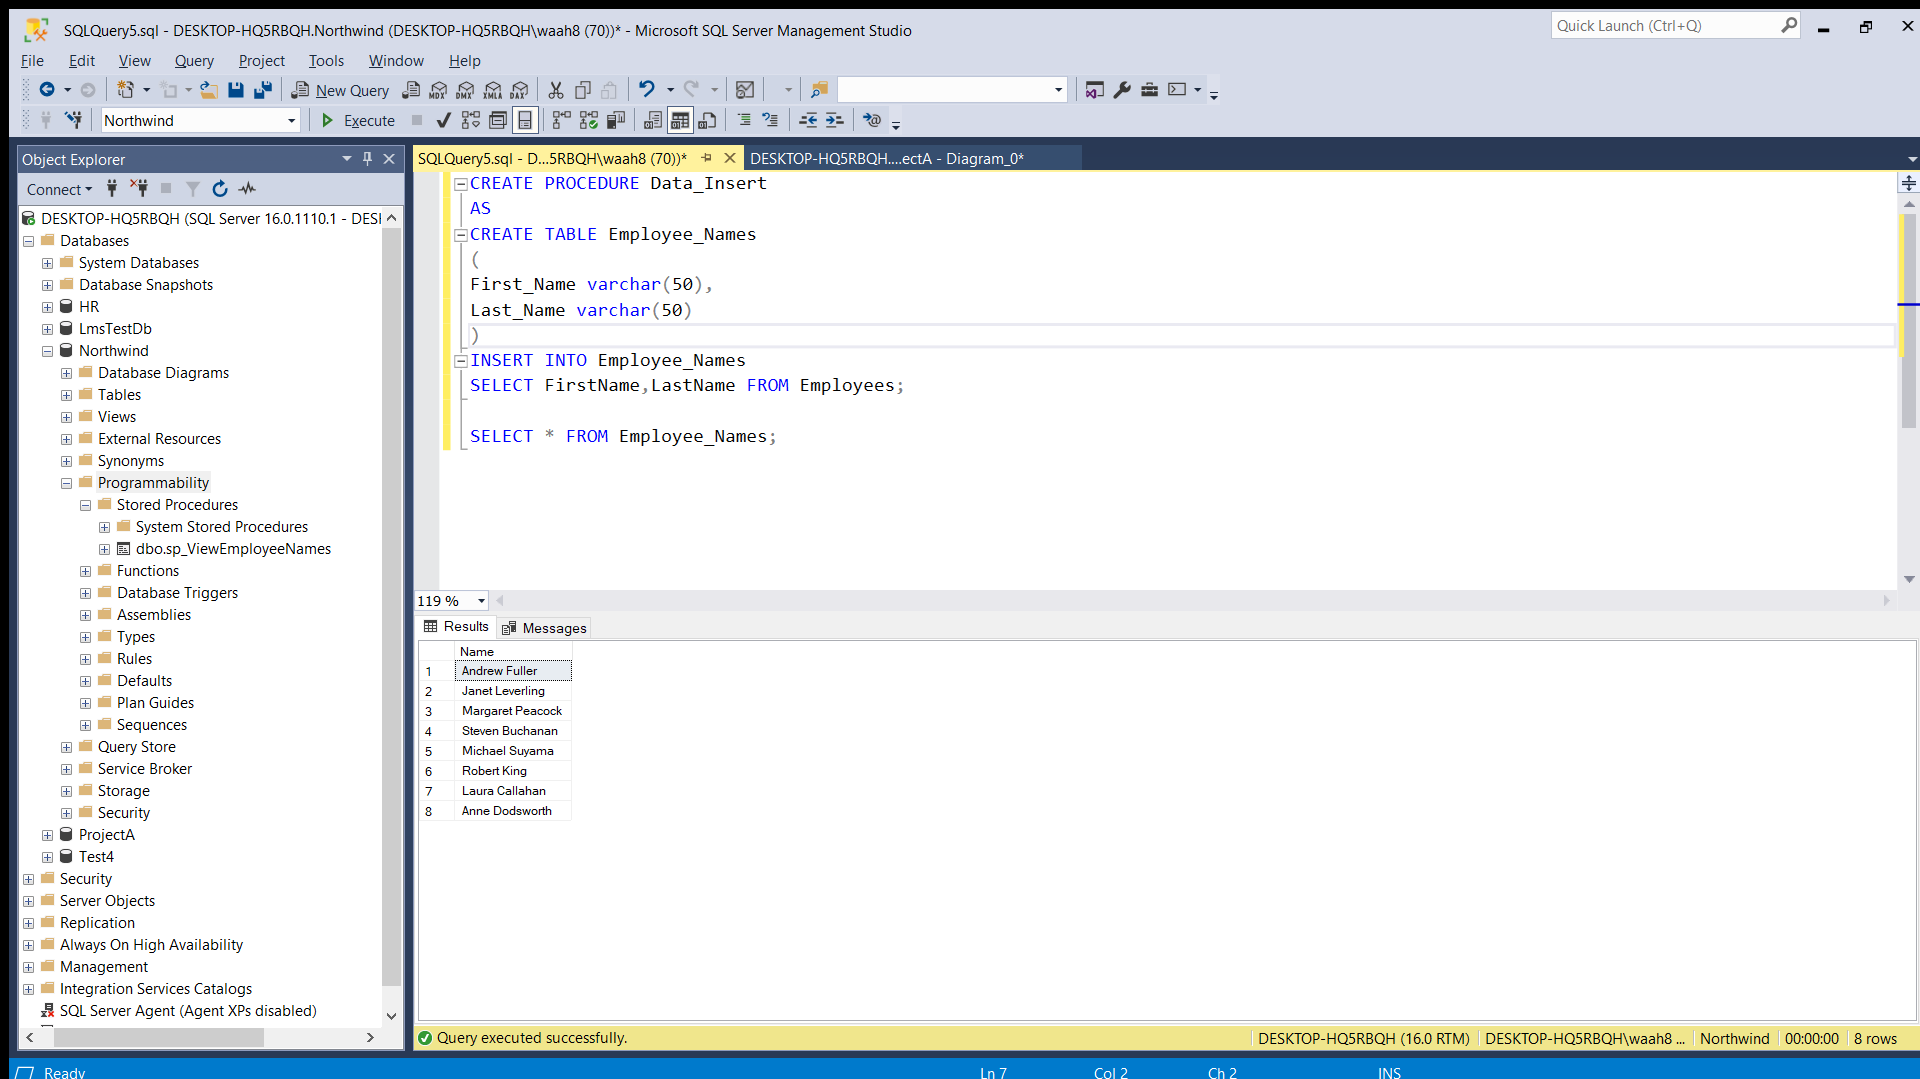
\includegraphics[width=1\textwidth]{6.png} \\
    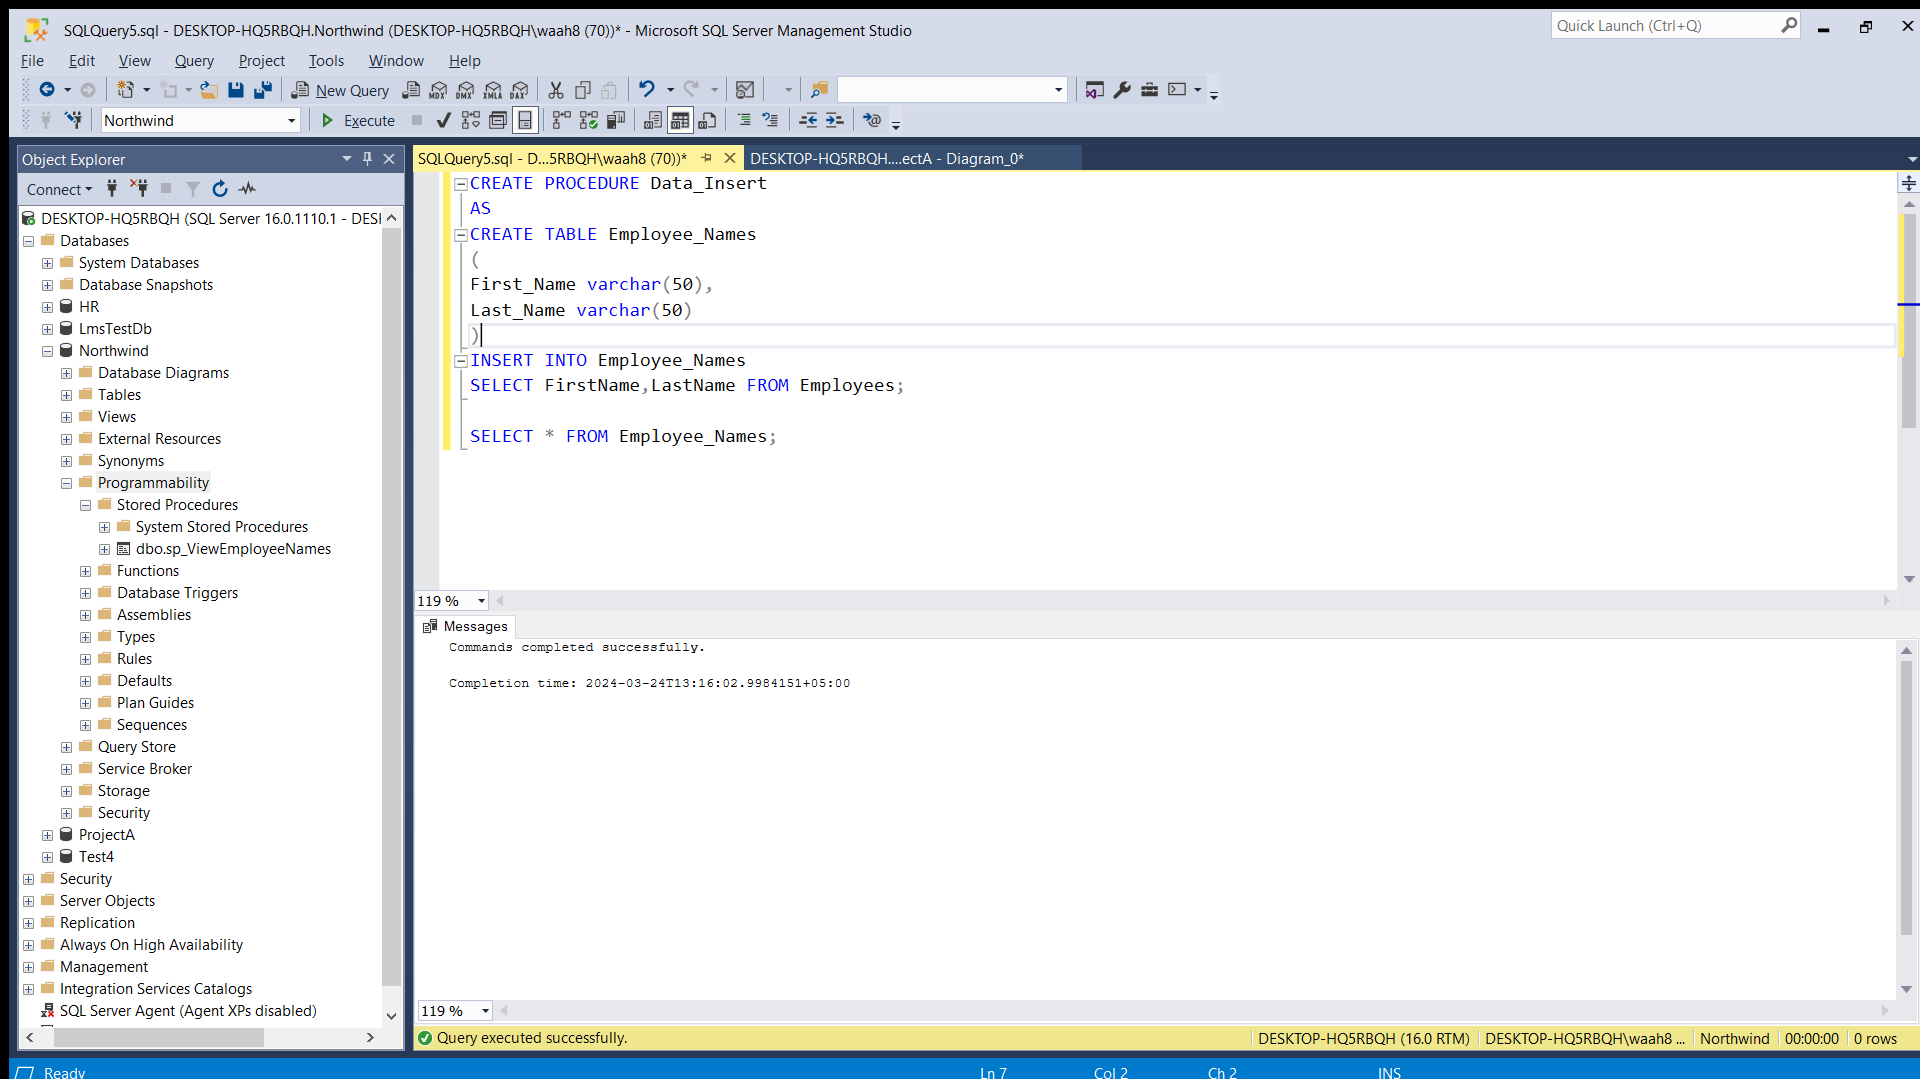
\includegraphics[width=1\textwidth]{7.png} \\
    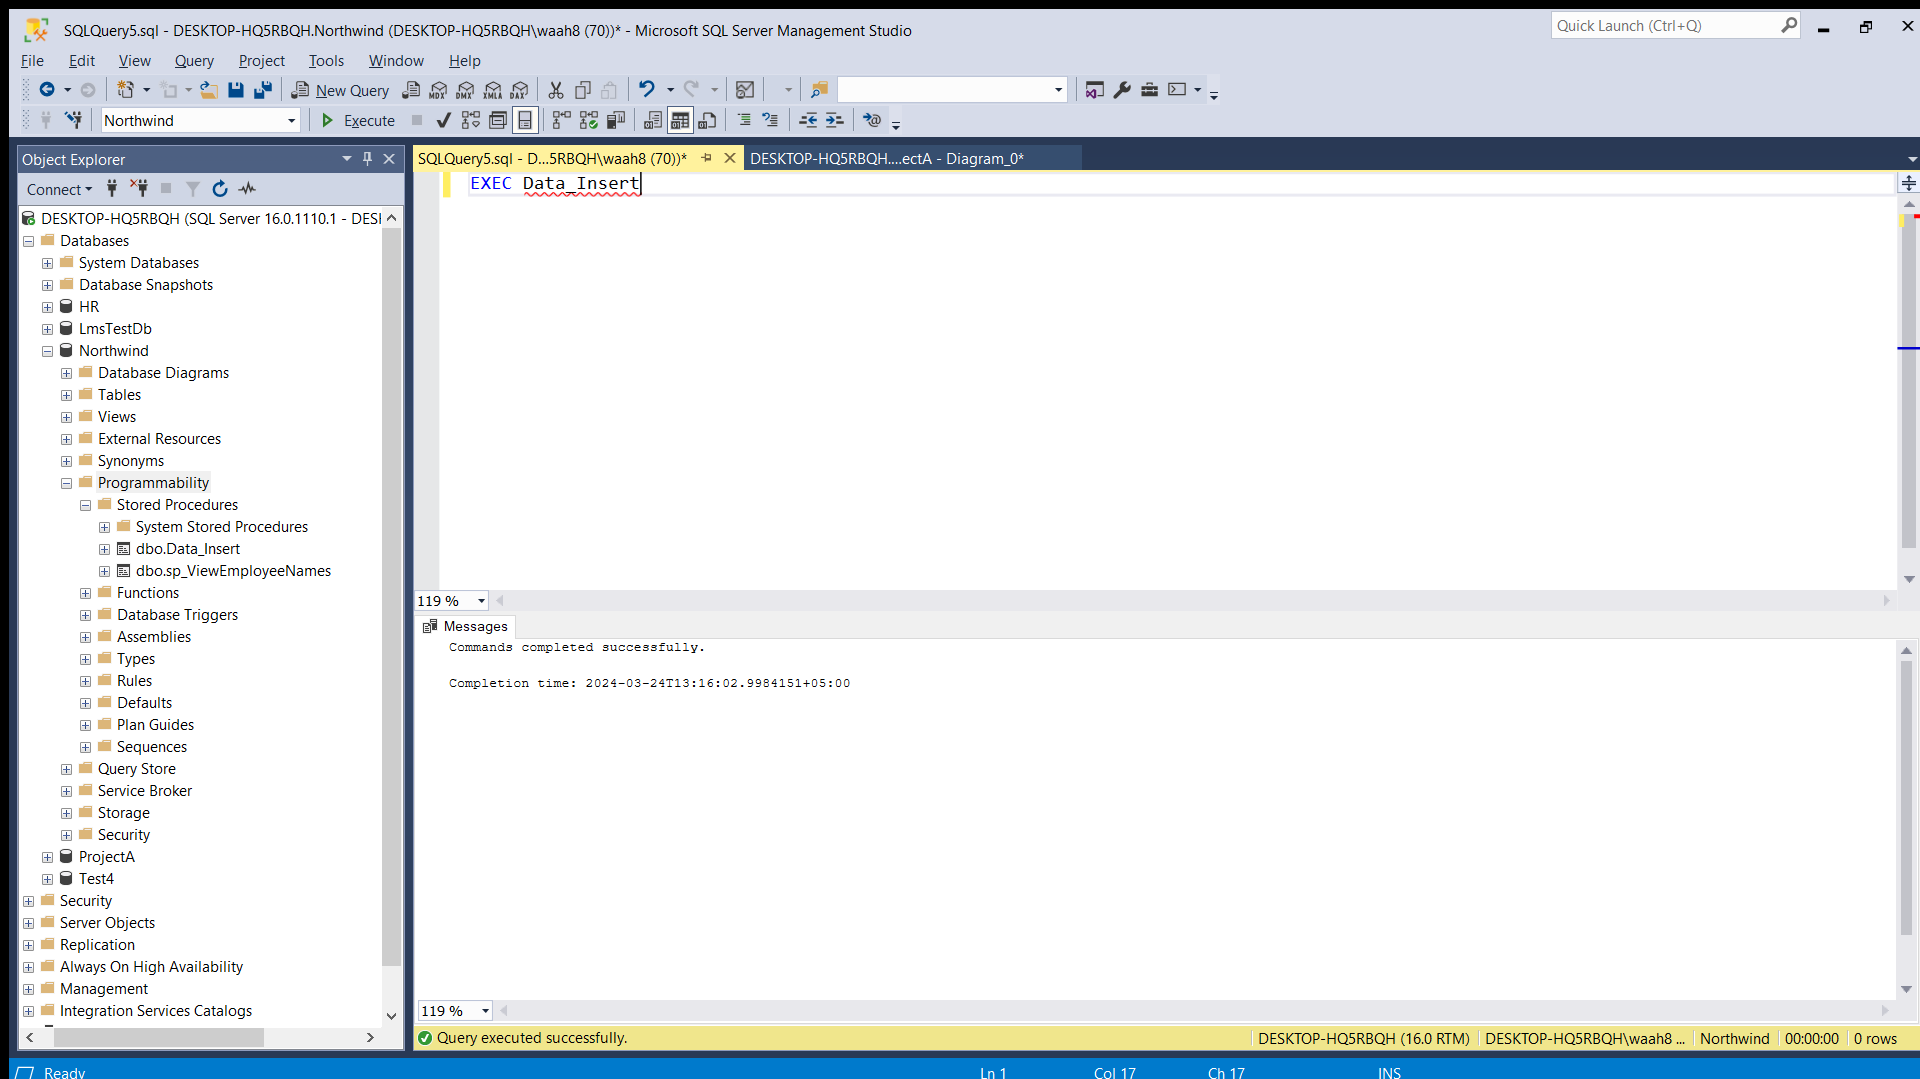
\includegraphics[width=1\textwidth]{8.png} \\
    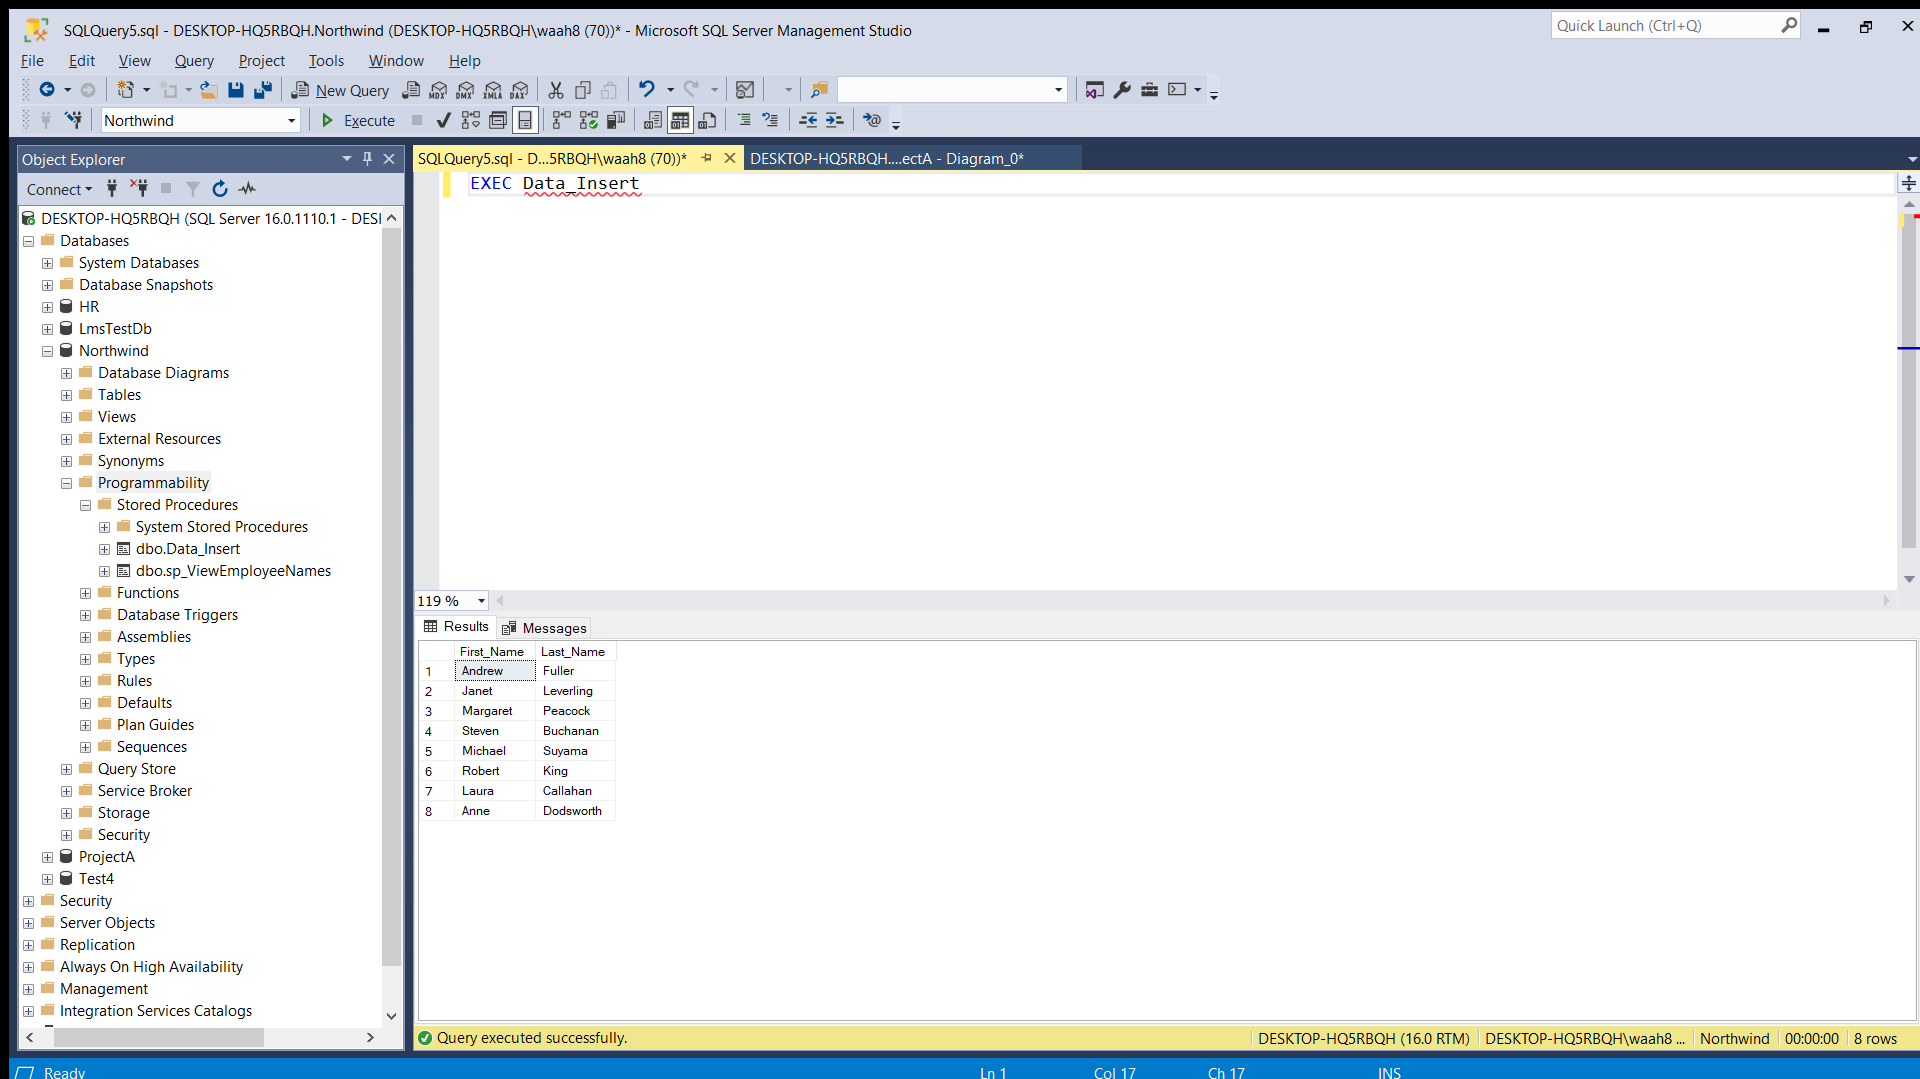
\includegraphics[width=1\textwidth]{9.png} \\
    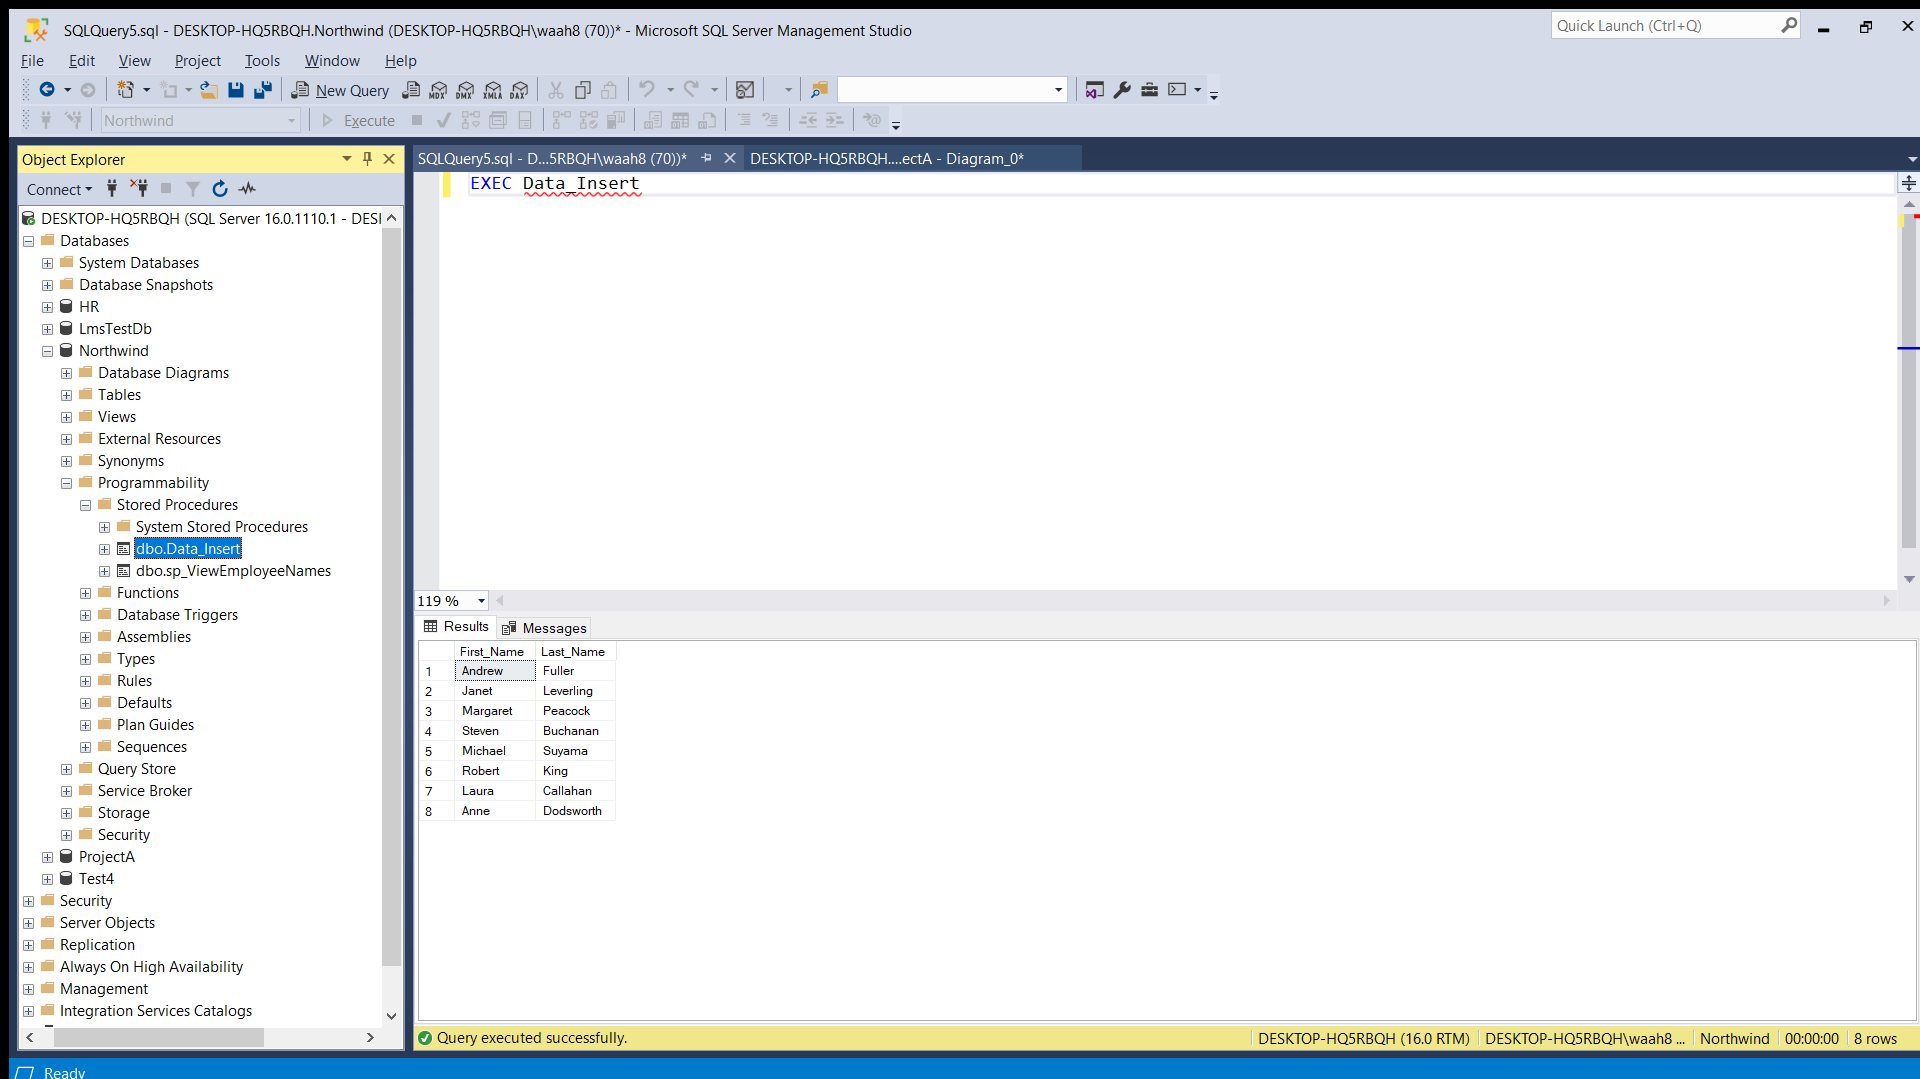
\includegraphics[width=1\textwidth]{10.png} \\
    \newpage 
    There is also another method to create a stored procedure that can only be accessed if it is only given the required parameters as specified in the stored query. A parametered stored query can be created by using \textbf{CREATE OR ALTER StoredProcedureName @Parameter}. The specified parameter may or may not be used in the query inside stored procedure. \\
    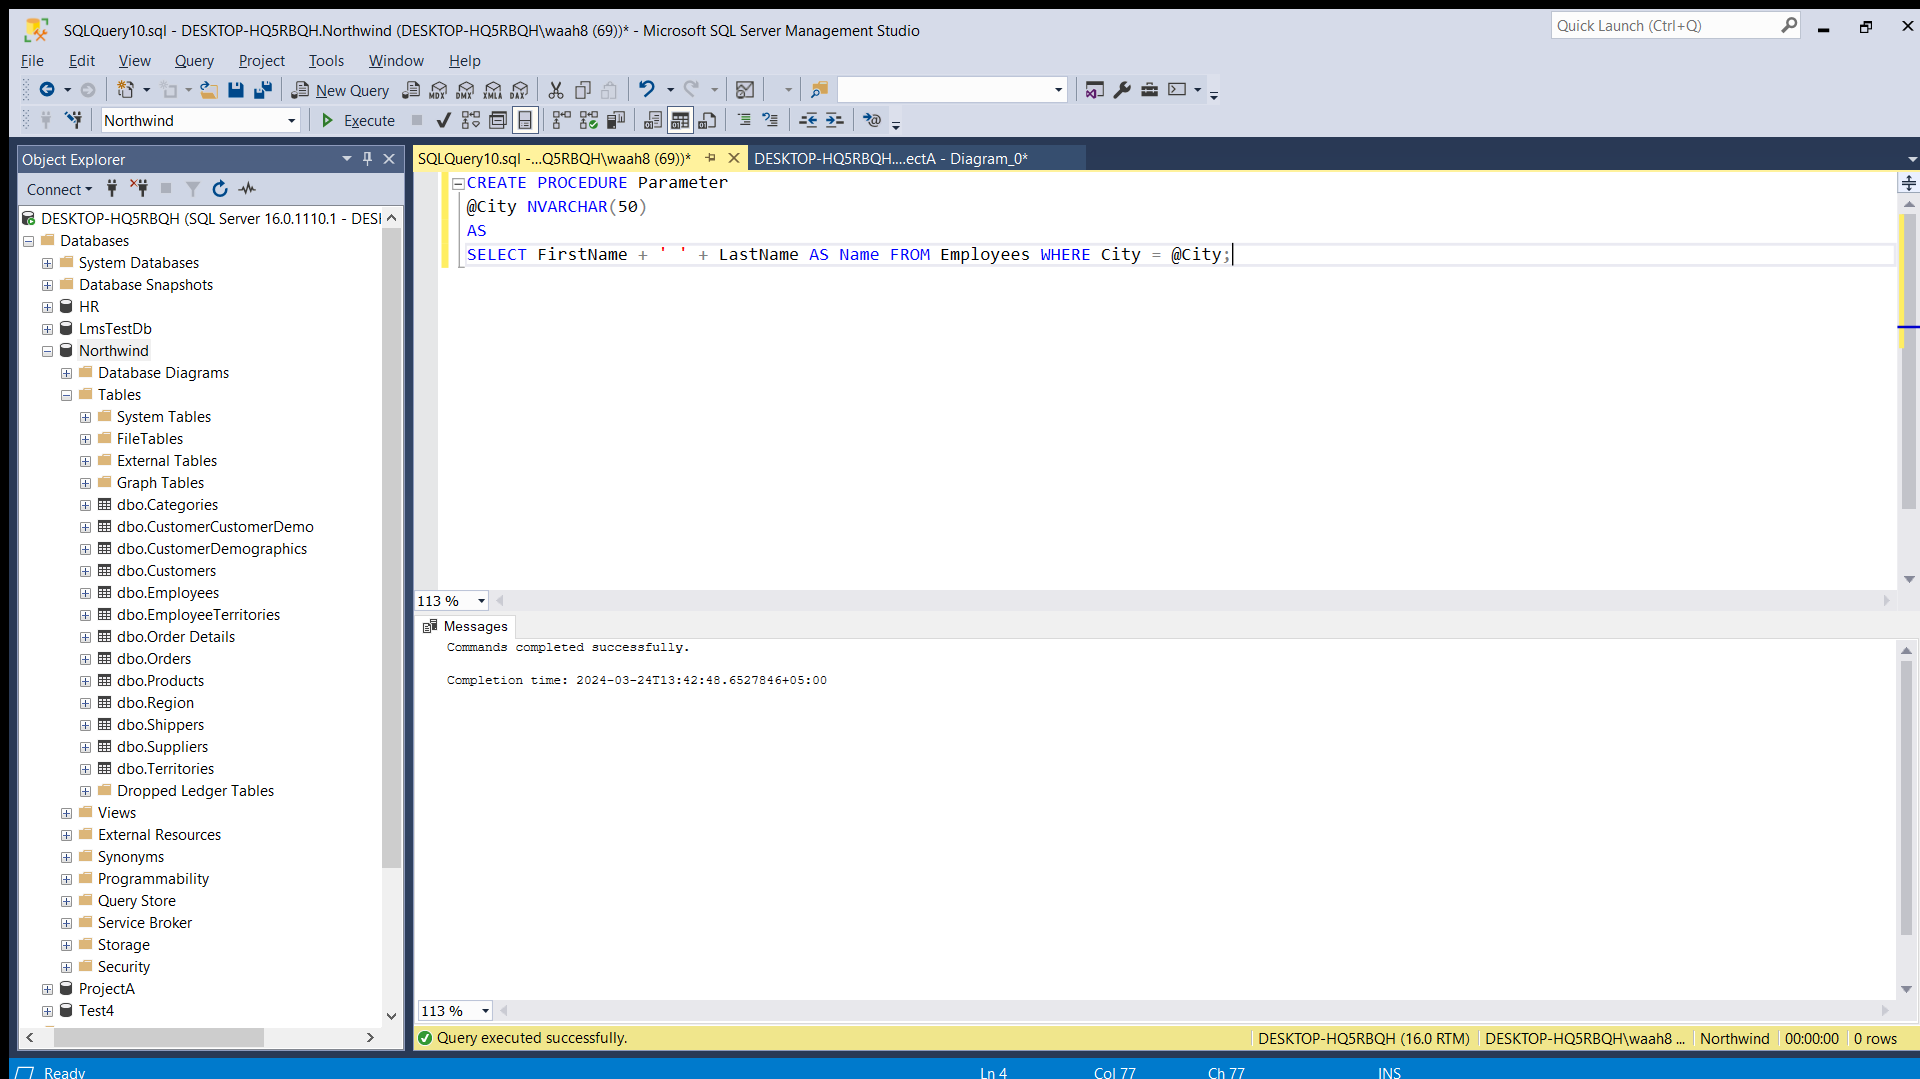
\includegraphics[width=1\textwidth]{11.png} \\
    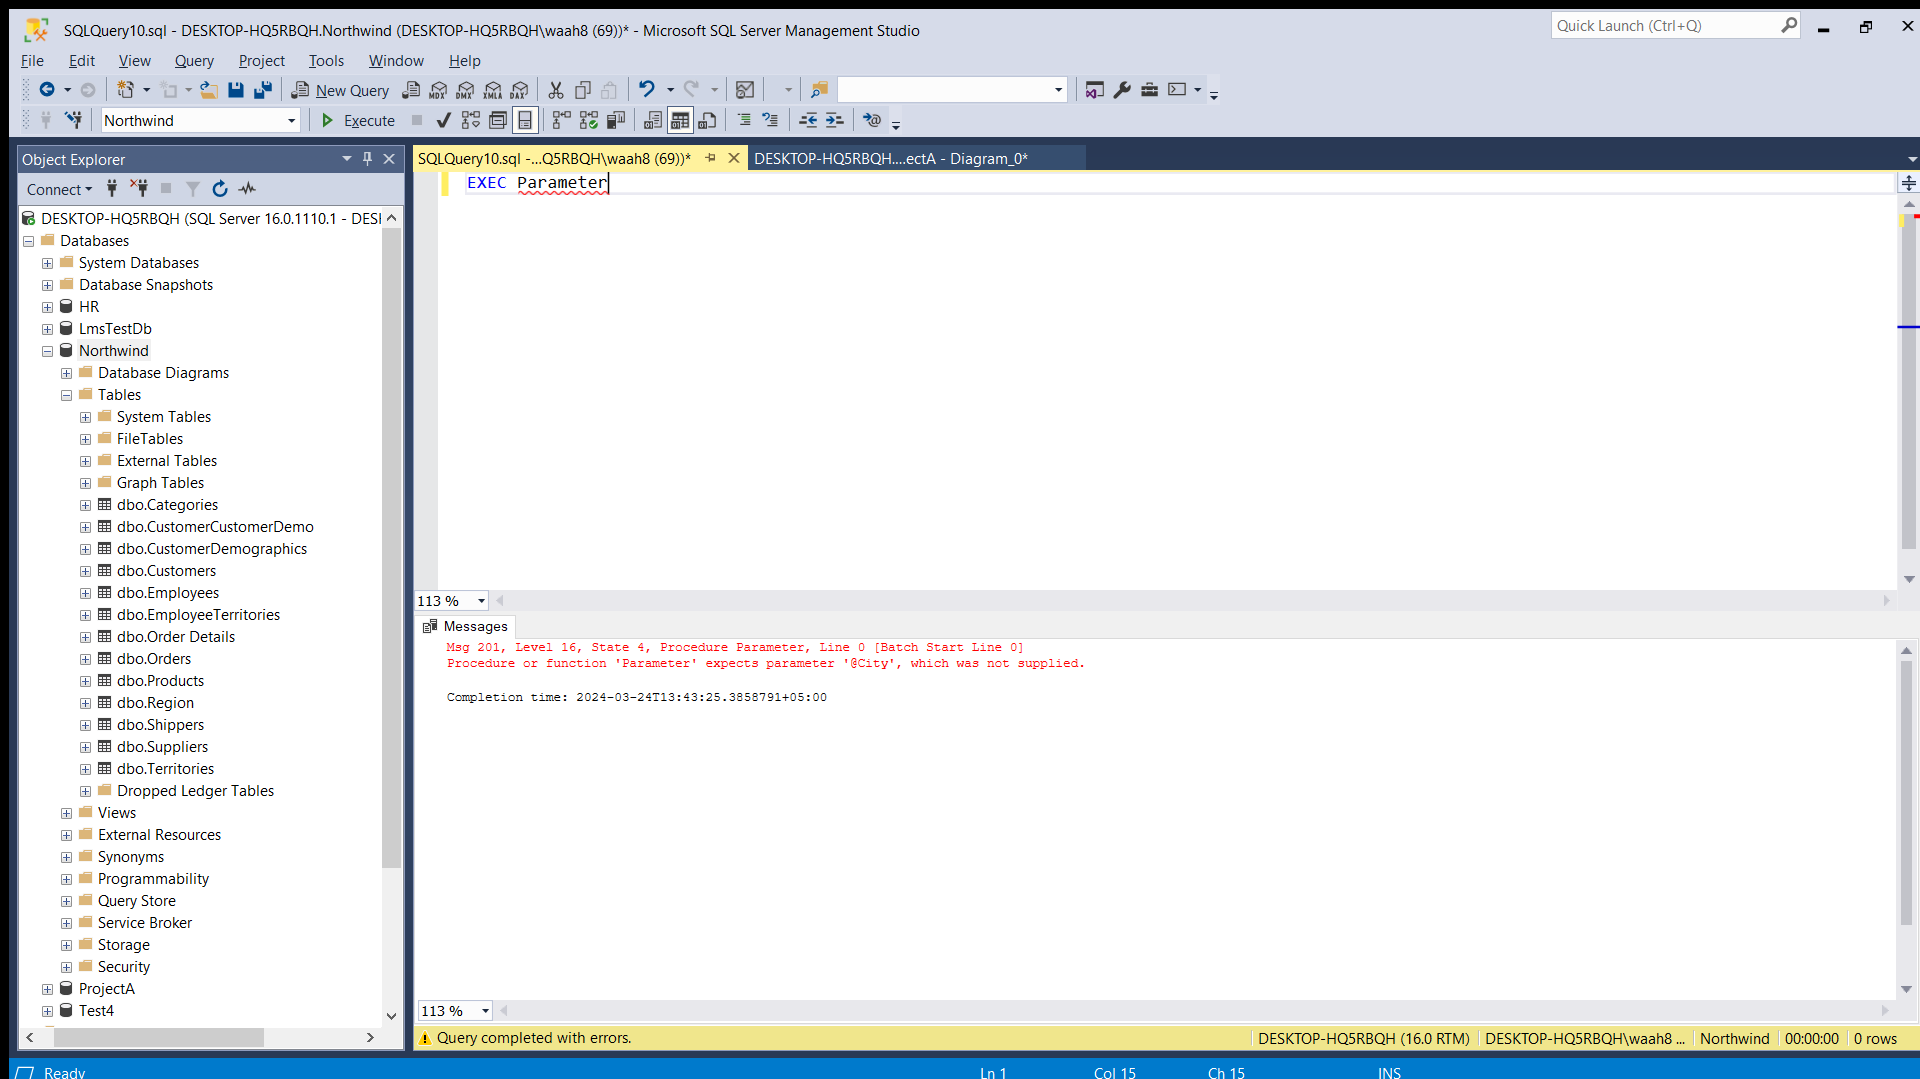
\includegraphics[width=1\textwidth]{12.png} \\
    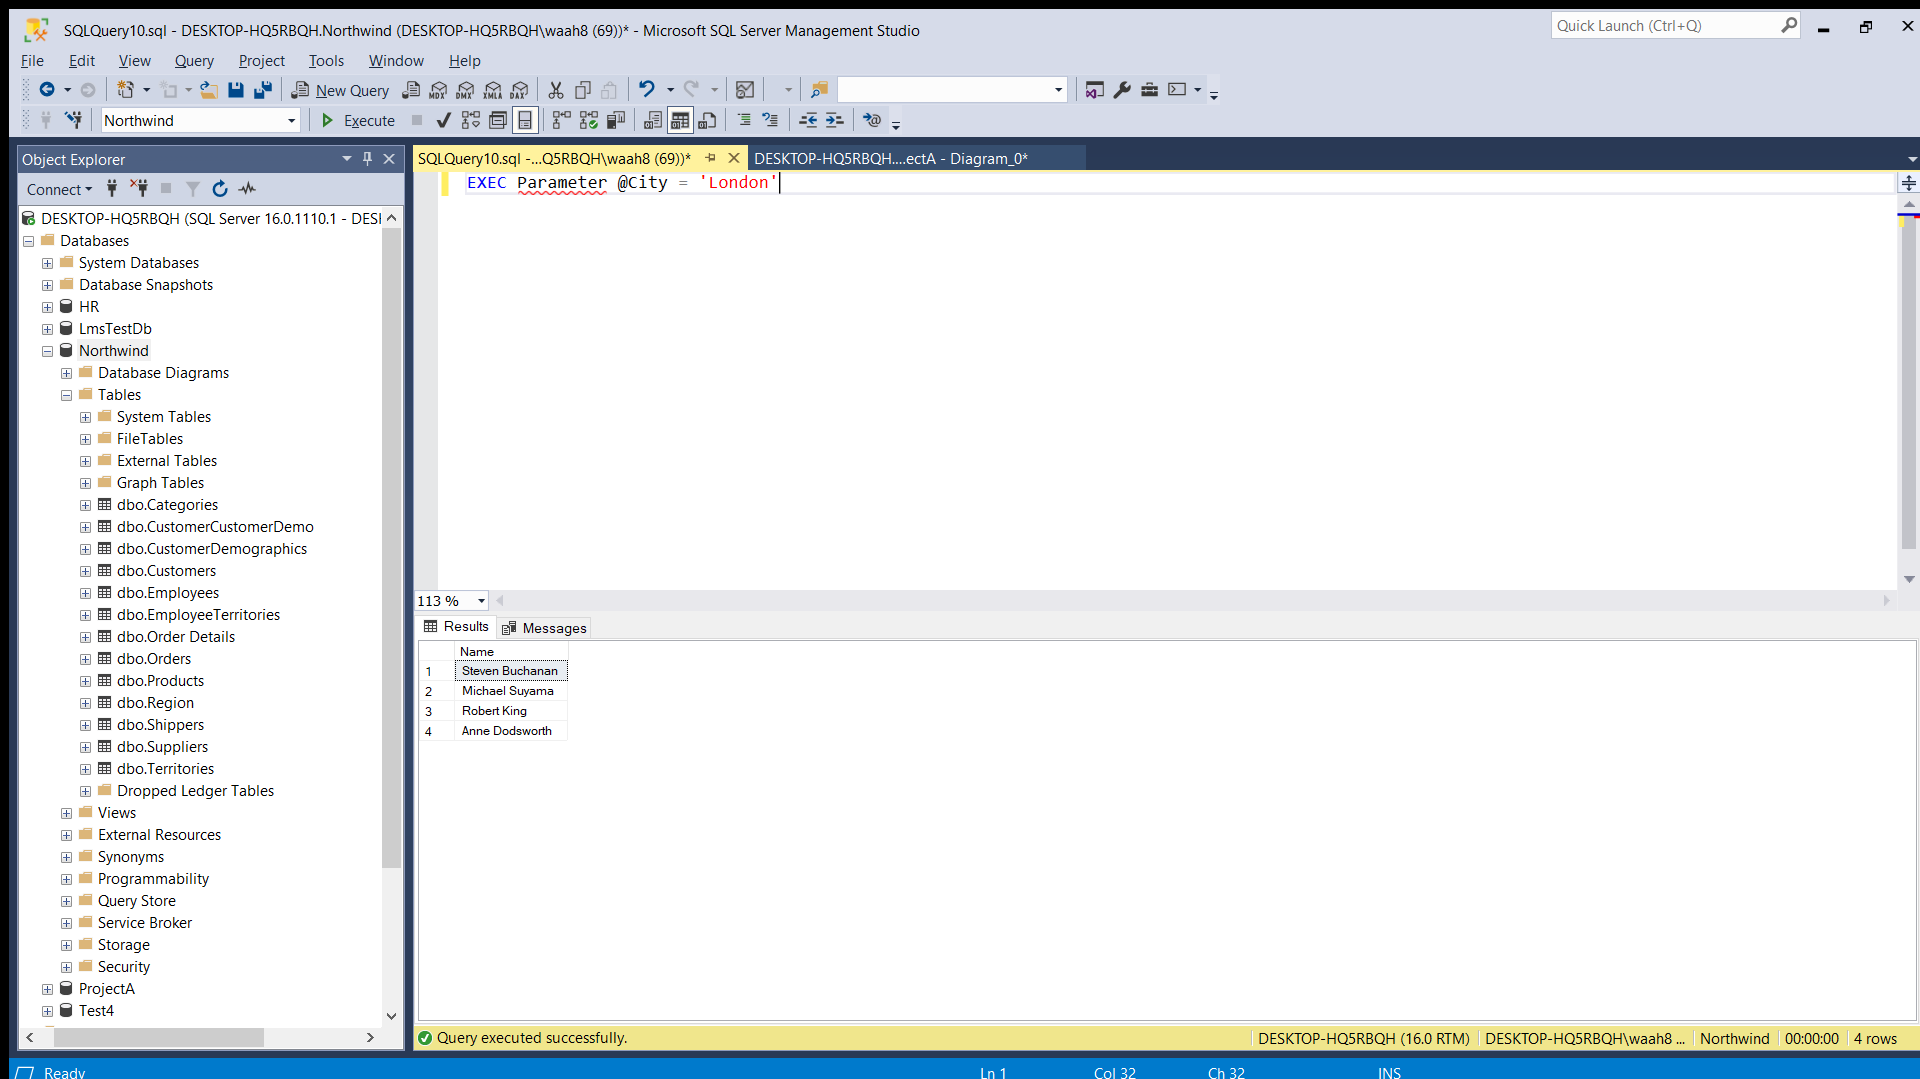
\includegraphics[width=1\textwidth]{13.png} \\
    It is inpportant to note that a parametered stored procedure will not execute if the parameter is not passed.
\end{center}
\end{document}
